% Progress update slide deck (Beamer)
% Compile (example): pdflatex picopatt_progress_2026-04-24.tex

\documentclass[aspectratio=169]{beamer}

\usetheme{Madrid}
\usecolortheme{default}

\usepackage{amsmath}
\usepackage{booktabs}
\usepackage{graphicx}
\usepackage{tikz}
\usetikzlibrary{positioning,arrows.meta,fit}

\graphicspath{{figures/}}

\title[Progress update]{PICOPATT progress update}
\subtitle{Simulated picoclimate testing, stability, and baseline expansion}
\institute{LIRMM}
\date{24 Apr 2026}

\begin{document}

\begin{frame}
  \titlepage
\end{frame}

\begin{frame}{Scope reminder}
  \begin{block}{Current data status}
    I still do not have the real PICOPATT data. The picoclimate work in the repository is a simulated test fixture used for validation only.
  \end{block}
  \vspace{0.5em}
  \begin{itemize}
    \item Simulated picoclimate fixture: 4 timesteps, about 23 variables, used to test the pipeline structure.
    \item Real PICOPATT validation remains future work once the real data is available.
    \item Current focus: keep the explanation format stable and broaden the benchmark matrix.
  \end{itemize}
\end{frame}

\begin{frame}{What changed recently}
  \begin{columns}[T,onlytextwidth]
    \column{0.52\textwidth}
    \begin{block}{Validated in code}
      \begin{itemize}
        \item Shapelet notebooks renamed and aligned under \texttt{shapelets\_}
        \item Cross-dataset stability run completed with 7 seeds
        \item HDBSCAN added to the picoclimate benchmark script
        \item Autoencoder + KMeans baseline already available and runnable
      \end{itemize}
    \end{block}

    \column{0.45\textwidth}
    \begin{block}{Governance update}
      \begin{itemize}
        \item Explanation output format is now treated as a contract
        \item Future methods must emit the same cluster-summary structure
        \item The goal is sensor-readable explanations, not feature-index-only narratives
      \end{itemize}
    \end{block}
  \end{columns}
\end{frame}

\begin{frame}{Evidence: stability across datasets}
  \begin{figure}
    \centering
    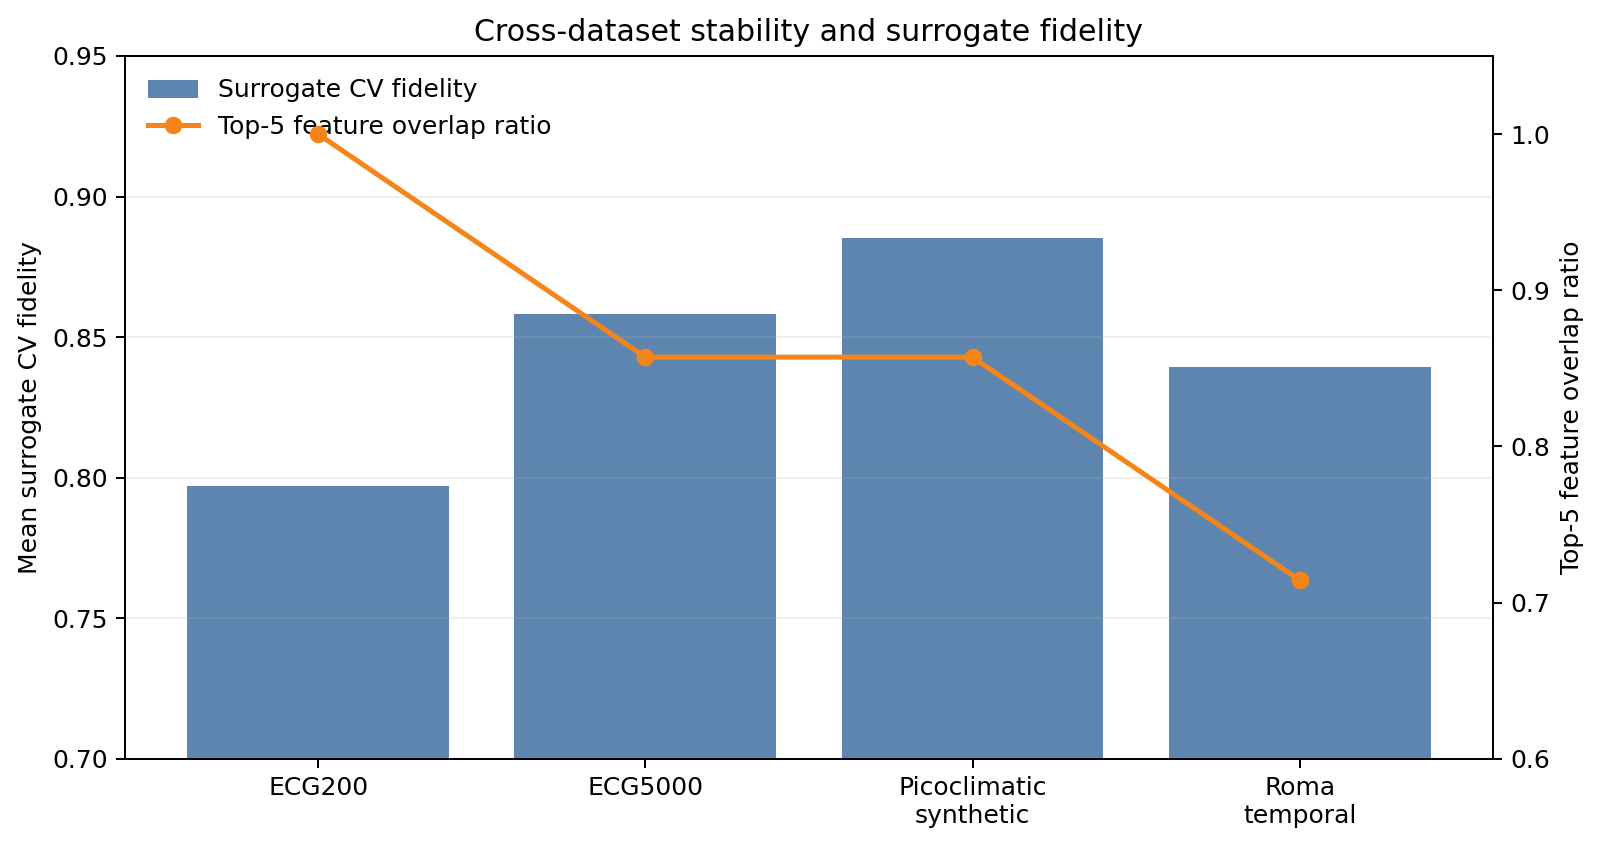
\includegraphics[width=0.92\linewidth]{stability_summary.png}
  \end{figure}
  \vspace{-0.7em}
  \begin{itemize}
    \item Surrogate CV fidelity stays roughly in the 0.80--0.89 band.
    \item Top-5 explanation overlap remains strong across 7 seeds.
    \item This is the main robustness evidence supporting the current explainability claim.
  \end{itemize}
\end{frame}

\begin{frame}{Evidence: deep representation baseline}
  \begin{figure}
    \centering
    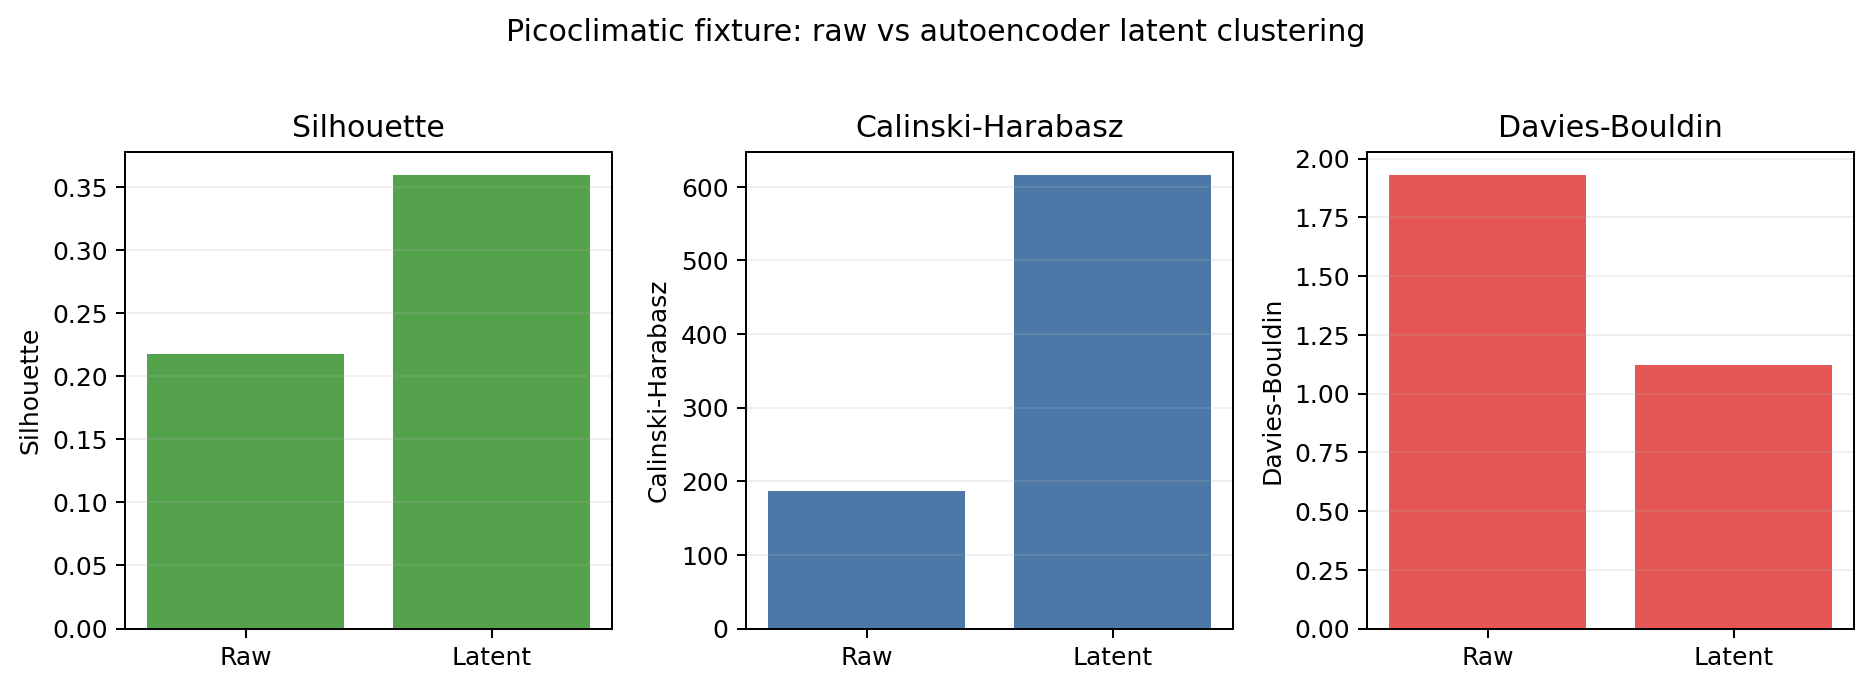
\includegraphics[width=0.95\linewidth]{deep_representation_comparison.png}
  \end{figure}
  \vspace{-0.6em}
  \begin{itemize}
    \item The autoencoder baseline already existed in the repository and is now validated on the simulated picoclimate fixture.
    \item Latent space improves clustering quality over the raw feature baseline in this quick test.
    \item This gives a concrete representation-space comparator for the next phase.
  \end{itemize}
\end{frame}

\begin{frame}{Evidence: spatial baseline expansion}
  \begin{figure}
    \centering
    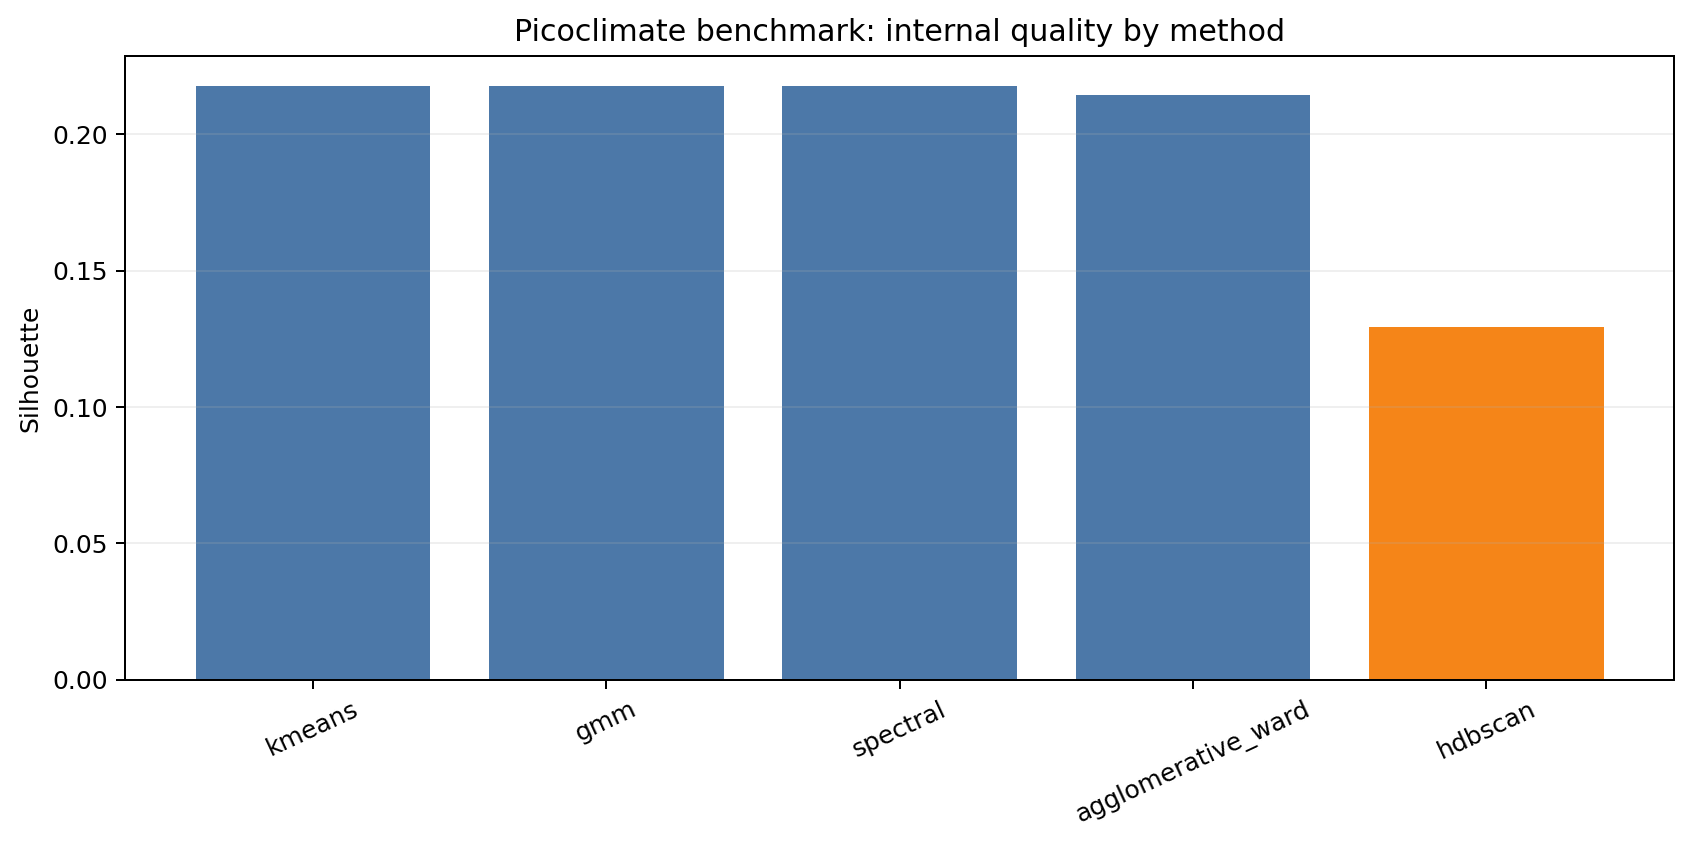
\includegraphics[width=0.95\linewidth]{benchmark_silhouette.png}
  \end{figure}
  \vspace{-0.6em}
  \begin{itemize}
    \item HDBSCAN is now part of the picoclimate benchmark script.
    \item This broadens the baseline set beyond KMeans / ExKMC.
    \item The benchmark is still a validation fixture, not the final PICOPATT benchmark.
  \end{itemize}
\end{frame}

\begin{frame}{Interpretation layer}
  \begin{columns}[T,onlytextwidth]
    \column{0.48\textwidth}
    \begin{block}{What is already supported}
      \begin{itemize}
        \item Surrogate fidelity is high enough to defend model-faithful explanations.
        \item SHAP concentration already gives a compact narrative for the shapelet baseline.
        \item Stability is now measured rather than assumed.
      \end{itemize}
    \end{block}

    \column{0.48\textwidth}
    \begin{block}{What is still missing}
      \begin{itemize}
        \item Sensor-unit explanation template frozen across methods
        \item Spatial density comparators on real PICOPATT data
        \item A fuller joint-optimization method if the paper goes beyond a pipeline story
      \end{itemize}
    \end{block}
  \end{columns}
\end{frame}

\begin{frame}{Recommended next phase}
  \begin{enumerate}
    \item Freeze the explanation output format and make every method emit the same cluster-summary schema.
    \item Keep ExKMC as the main interpretable clustering baseline for now.
    \item Extend the benchmark matrix with spatial methods; HDBSCAN is the first one now in place.
    \item Treat the autoencoder + KMeans path as the deep representation baseline.
    \item If the research contribution shifts toward methods, prototype the simplified ExKMC-style spatial regularizer next.
  \end{enumerate}

  \vspace{0.5em}
  \begin{block}{Practical takeaway}
    The current repository is now ready for a Phase 2 story: simulated validation, stable explanations, and broader clustering baselines before moving to real PICOPATT data.
  \end{block}
\end{frame}

\begin{frame}{Slide space for future figures}
  \begin{block}{Reserved space}
    \vspace{1em}
    \centering
    \fbox{\parbox{0.82\linewidth}{\vspace{2.2cm}\centering\small Reserved for future PICOPATT cluster visualizations, sensor-readable summaries, or spatial maps.\vspace{2.2cm}}}
  \end{block}

  \vspace{0.6em}
  \footnotesize Suggested future figures: cluster profile heatmap, station map, and one explanation example with sensor units.
\end{frame}

\end{document}